% Provenance (never printed): old premiere S / seconde material on minerals and
% rocks (identifying minerals in hand specimen, the silicates, the minerals of
% granite, basalt and peridotite, thin sections in polarised light).
% Element fractions and rock densities from figdata/grade-11/mineral_density.py
% (Rudnick and Gao 2014 bulk crust; webmineral mean densities). Mineral, crystal,
% rock families and the Mohs scale are Book 1's (grade 6): recalled, not defined.
% Felsic and mafic belong to g11.08: not used here.
\chapter{Minerals}\label{ch:g11:minerals}

Pick up a granite pebble and look at it through a hand lens. It is not one
substance but a mosaic of grains locked together: grey grains, glassy and
almost transparent; pink grains, blocky, whose broken faces flash in the
light when the pebble is turned; small black flakes that a knife tip lifts
off in thin sheets. Each kind of grain is a mineral. This chapter shows how
a geologist tells them apart, why almost all of them are built from silicon
and oxygen, how they make the rocks met so far --- granite, basalt,
\omterm{def:g11:ocean-ridges:peridotite}{peridotite} --- and how a slice of rock thinner than a hair, seen in polarised
light, shows them all at once.

\begin{omfigure}
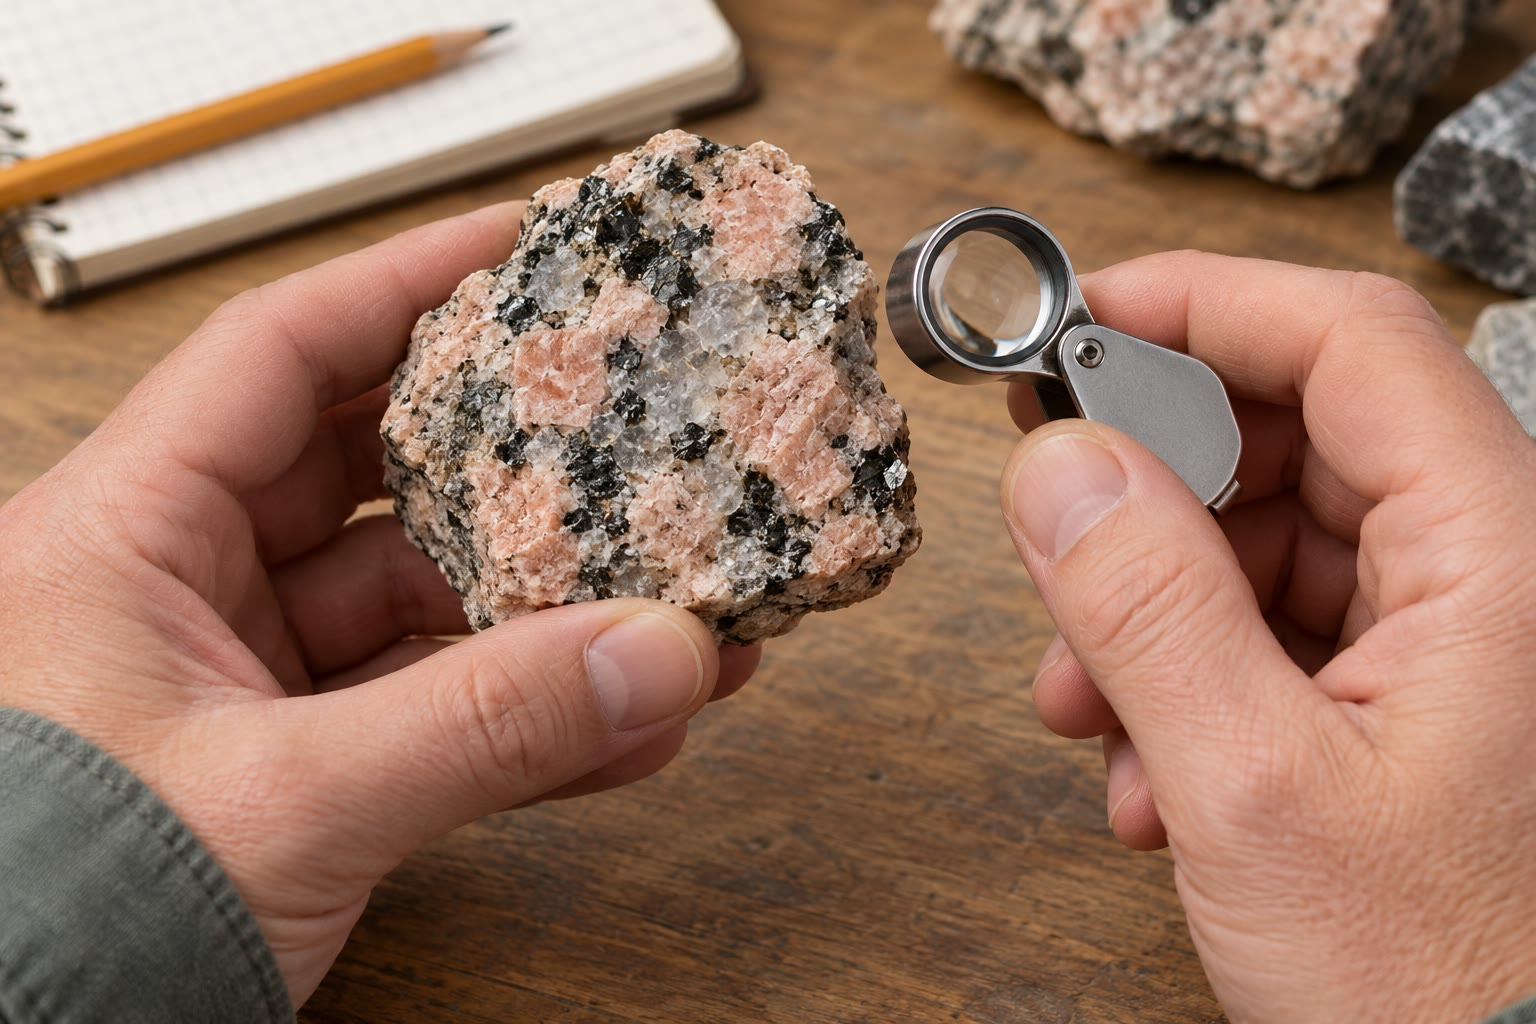
\includegraphics[width=0.62\linewidth]{images/book2/ai/g11-geologist-hand-lens.jpg}

{\small A granite examined with a hand lens: the first tool for telling
minerals apart. (AI-generated illustration.)}
\end{omfigure}

\begin{recall}
A mineral is a natural solid substance, not made by living things, with a
fixed make-up and its atoms arranged in a regular way; a rock is made of one
or several minerals. Granite is made mostly of feldspar, quartz and mica.
Rocks fall into three families, igneous, sedimentary and metamorphic. The
hardness of a mineral is how well it resists being scratched, ranked from 1
(talc) to 10 (diamond) on the Mohs scale; orthoclase feldspar is 6 and quartz
7, while a glass plate is about 5.5 and a steel nail about 6.5 (Book 1,
grade 6). The density of a body is its mass divided by its volume
(physics). A compound is described by a formula that counts its atoms; in a
solid made of ions, the positive and negative charges balance (chemistry).
\omterm{def:g11:ocean-ridges:peridotite}{Peridotite} makes the mantle; \omterm{def:g11:ocean-ridges:gabbro}{gabbro} and basalt make the \omterm{def:g11:ocean-ridges:oceanic-lithosphere}{oceanic crust}
(\cref{ch:g11:ocean-ridges}).
\end{recall}
% ledger: usgs:mineral-rock, nps:granite-minerals, nps:mohs-ladder, nps:mohs-testers

\section{Telling minerals apart}

A mineral has a fixed make-up and a regular arrangement of atoms. Both show
on the outside: in the shape of its crystals, the way it breaks, the way it
reflects light, its hardness and its density. None of these properties is
enough alone; together they identify the common minerals in a hand specimen,
with no instrument but a lens, a steel nail and a glass plate.

\paragraph{Shape.} A crystal that grew freely, in a cavity or in a liquid,
takes a shape that reflects the arrangement of its atoms.

\begin{definition}[Habit]\label{def:g11:minerals:habit}
The \emph{habit}\index{habit (of a crystal)} of a mineral is the general shape
its crystals take: cubic, tabular (flat, like a tablet), prismatic
(elongated, like a prism), bladed, acicular (needle-like), and so on.
\end{definition}
% ledger: tulane:physprop

Quartz grows as six-sided prisms ending in points; biotite, as flat
six-sided plates (photographs below). In most rocks, though, the grains grew
against one another and have no faces of their own: \omterm{def:g11:minerals:habit}{habit} then tells little,
and the other properties take over.
% ledger: photo:g11-quartz, photo:g11-biotite

\paragraph{Colour and lustre.} Colour is the first thing one sees, and the
least reliable. A trace of another element is enough to change it: quartz
can be clear, white, black, pink, blue or purple. A few minerals, on the
other hand, hardly vary: olivine is almost always green. How a mineral
reflects light is a better guide.
% ledger: tulane:physprop

\begin{definition}[Lustre]\label{def:g11:minerals:lustre}
The \emph{lustre}\index{lustre} of a mineral is its appearance in reflected
light. It is \emph{metallic} when the mineral shines like a metal, and
non-metallic otherwise: \emph{vitreous} (glassy, like quartz), pearly,
resinous, and so on.
\end{definition}
% ledger: tulane:physprop

\paragraph{The way it breaks.} Strike a crystal and it breaks. Where the
bonds between its atoms are weaker along certain planes, it splits along
them, again and again, into flat shining surfaces; where no plane is weaker
than another, it breaks along any surface.

\begin{definition}[Cleavage; fracture]\label{def:g11:minerals:cleavage}
\emph{Cleavage}\index{cleavage (of a mineral)} is the tendency of a mineral
to break along flat planes, parallel to directions in which the bonds
between its atoms are weaker. \emph{Fracture}\index{fracture (of a mineral)}
is breakage along irregular surfaces, in a mineral with no plane of
weakness; a fracture with smooth curved surfaces, like broken glass, is
called \emph{conchoidal}.
\end{definition}
% ledger: tulane:physprop

A mineral may have one \omterm{def:g11:minerals:cleavage}{cleavage}, two, three or none. Micas have one, perfect:
they peel into sheets. Feldspars have two. Quartz has none: it breaks with a
conchoidal fracture, which tells it at once from a feldspar of the same grey
or white colour. The angle between two \omterm{def:g11:minerals:cleavage}{cleavages} is fixed by the arrangement
of the atoms, and it can be measured on a broken grain or a section: the two
\omterm{def:g11:minerals:cleavage}{cleavages} of a pyroxene meet at about \ang{87} and \ang{93}, nearly a right
angle; those of an amphibole at about \ang{56} and \ang{124}. Pyroxenes and
amphiboles are often dark and alike; their \omterm{def:g11:minerals:cleavage}{cleavage} angles tell them apart.
% ledger: wm:densities (quartz conchoidal; orthoclase two cleavages; biotite one), tulane:cleavage-angles

\begin{omfigure}
\begin{tikzpicture}[font=\footnotesize]
  % pyroxene: octagonal cross-section, cleavage traces at 46.5 and 133.5 degrees (87/93)
  \begin{scope}
    \coordinate (p1) at (1,0.4); \coordinate (p2) at (0.431,1); \coordinate (p3) at (-0.431,1);
    \coordinate (p4) at (-1,0.4); \coordinate (p5) at (-1,-0.4); \coordinate (p6) at (-0.431,-1);
    \coordinate (p7) at (0.431,-1); \coordinate (p8) at (1,-0.4);
    \begin{scope}[scale=1.5]
      \fill[black!72!green!40] (1,0.4) -- (0.431,1) -- (-0.431,1) -- (-1,0.4) -- (-1,-0.4) -- (-0.431,-1) -- (0.431,-1) -- (1,-0.4) -- cycle;
      \clip (1,0.4) -- (0.431,1) -- (-0.431,1) -- (-1,0.4) -- (-1,-0.4) -- (-0.431,-1) -- (0.431,-1) -- (1,-0.4) -- cycle;
      \foreach \s in {-5,...,5} {
        \draw[white!85!black, line width=0.5pt] ($(136.5:\s*0.24)+(46.5:-3)$) -- ($(136.5:\s*0.24)+(46.5:3)$);
        \draw[white!85!black, line width=0.5pt] ($(223.5:\s*0.24)+(133.5:-3)$) -- ($(223.5:\s*0.24)+(133.5:3)$);}
      \draw[black!80, line width=0.9pt] (46.5:-3) -- (46.5:3); \draw[black!80, line width=0.9pt] (133.5:-3) -- (133.5:3);
    \end{scope}
    \draw[black!70, line width=0.7pt, scale=1.5] (1,0.4) -- (0.431,1) -- (-0.431,1) -- (-1,0.4) -- (-1,-0.4) -- (-0.431,-1) -- (0.431,-1) -- (1,-0.4) -- cycle;
    \draw[omProp, line width=1pt] (46.5:0.75) arc[start angle=46.5, end angle=133.5, radius=0.75];
    \draw[omDef, line width=1pt] (133.5:0.5) arc[start angle=133.5, end angle=226.5, radius=0.5];
    \node[fill=white, inner sep=1pt, text=omProp!80!black] at (90:0.98) {\ang{87}};
    \node[fill=white, inner sep=1pt, text=omDef] at (180:0.82) {\ang{93}};
    \node[anchor=north, align=center] at (0,-1.7) {\strut\textbf{pyroxene}\\cleavages at about \ang{87} and \ang{93}};
  \end{scope}
  % amphibole: elongated hexagon, cleavage traces at 28 and 152 degrees (56/124 opening sideways)
  \begin{scope}[xshift=6.2cm]
    \begin{scope}[scale=1.5]
      \fill[black!72!green!40] (1.6,0) -- (0.62,0.52) -- (-0.62,0.52) -- (-1.6,0) -- (-0.62,-0.52) -- (0.62,-0.52) -- cycle;
      \clip (1.6,0) -- (0.62,0.52) -- (-0.62,0.52) -- (-1.6,0) -- (-0.62,-0.52) -- (0.62,-0.52) -- cycle;
      \foreach \s in {-6,...,6} {
        \draw[white!85!black, line width=0.5pt] ($(118:\s*0.2)+(28:-4)$) -- ($(118:\s*0.2)+(28:4)$);
        \draw[white!85!black, line width=0.5pt] ($(242:\s*0.2)+(152:-4)$) -- ($(242:\s*0.2)+(152:4)$);}
      \draw[black!80, line width=0.9pt] (28:-4) -- (28:4); \draw[black!80, line width=0.9pt] (152:-4) -- (152:4);
    \end{scope}
    \draw[black!70, line width=0.7pt, scale=1.5] (1.6,0) -- (0.62,0.52) -- (-0.62,0.52) -- (-1.6,0) -- (-0.62,-0.52) -- (0.62,-0.52) -- cycle;
    \draw[omProp, line width=1pt] (-28:0.75) arc[start angle=-28, end angle=28, radius=0.75];
    \draw[omDef, line width=1pt] (28:0.42) arc[start angle=28, end angle=152, radius=0.42];
    \node[fill=white, inner sep=1pt, text=omProp!80!black] at (0:1.02) {\ang{56}};
    \node[fill=white, inner sep=1pt, text=omDef] at (90:0.6) {\ang{124}};
    \node[anchor=north, align=center] at (0,-1.7) {\strut\textbf{amphibole}\\cleavages at about \ang{56} and \ang{124}};
  \end{scope}
\end{tikzpicture}

{\small Cross-sections of a pyroxene crystal (left) and an amphibole crystal
(right), cut across their length (a drawing). The thin lines are the traces
of the two \omterm{def:g11:minerals:cleavage}{cleavages}, two of them drawn thicker where the angles are read;
the angles between them, nearly square in the pyroxene, much more open and much more closed in the amphibole, tell two
otherwise similar dark minerals apart.}
\end{omfigure}
% ledger: tulane:cleavage-angles

\paragraph{Hardness and density.} Hardness, met in Book 1, separates
minerals that look alike: quartz (7) scratches glass and is not scratched by
a steel nail; a feldspar (6) also scratches glass, but the nail scratches it.
Density is the last clue. In the hand, a grain cannot be weighed, but a
specimen of one mineral can, and the common minerals of rocks span a narrow
range, from about \qty{2.6}{g/cm^3} to about \qty{3.4}{g/cm^3} (chart below):
the lightest are rich in silicon, aluminium, sodium and potassium, the
densest in iron and magnesium.
% ledger: nps:mohs-ladder, nps:mohs-testers, wm:densities

\begin{method}[Identifying a mineral in hand specimen]\label{met:g11:minerals:identify}
\begin{enumerate}
  \item Look at the shape of the grain or crystal (\omterm{def:g11:minerals:habit}{habit}), its colour --- as
        a hint only --- and its \omterm{def:g11:minerals:lustre}{lustre}.
  \item Look for \omterm{def:g11:minerals:cleavage}{cleavage}: flat shining surfaces that catch the light
        together when the specimen is turned. Count the \omterm{def:g11:minerals:cleavage}{cleavage} directions
        and estimate the angle between them; if there is none, describe the
        fracture.
  \item Test the hardness against reference objects: a glass plate (about
        5.5) and a steel nail (about 6.5).
  \item If the specimen is a single mineral, compare its density with the
        densities of the candidates.
  \item Conclude by the combination of properties, never by one alone.
\end{enumerate}
\end{method}
% ledger: nps:mohs-testers

\begin{example}[Quartz or feldspar?]
Two grey-white grains in a granite. The first shows no flat face, only
smooth curved breaks, and the steel nail leaves no mark on it: conchoidal
fracture and a hardness above 6.5, it is quartz (7). The second breaks into
flat shining surfaces in two directions and is scratched by the nail, though
it scratches glass: two \omterm{def:g11:minerals:cleavage}{cleavages} and a hardness between 5.5 and 6.5, it is
a feldspar (6).
\end{example}
% ledger: wm:densities, nps:mohs-ladder, nps:mohs-testers

\begin{omfigure}
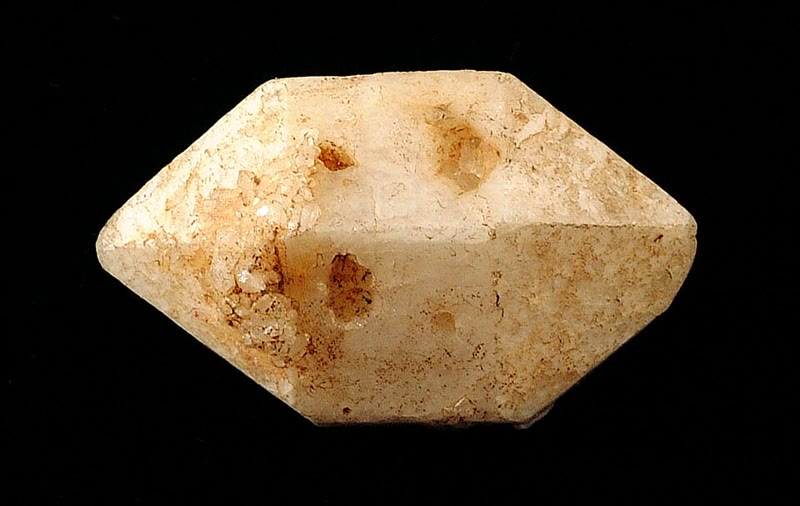
\includegraphics[height=2.75cm]{images/book2/g11-geodil-quartz.jpg}\hfill
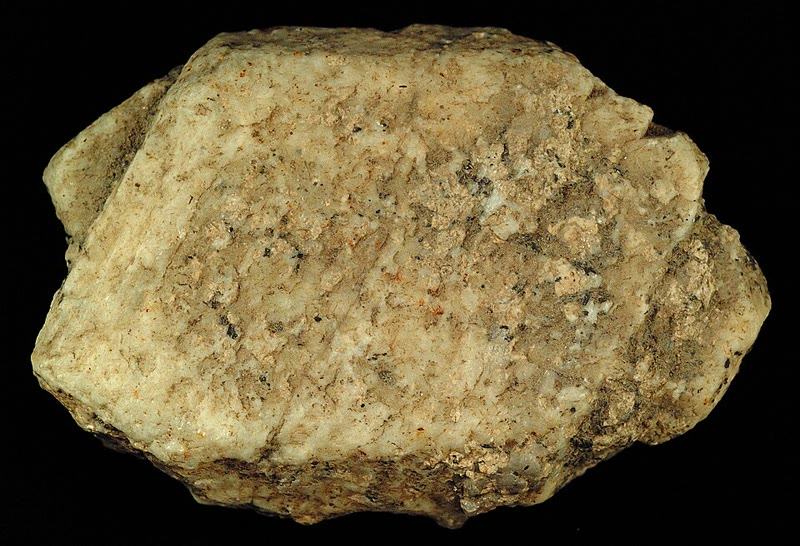
\includegraphics[height=2.75cm]{images/book2/g11-geodil-orthoclase.jpg}\hfill
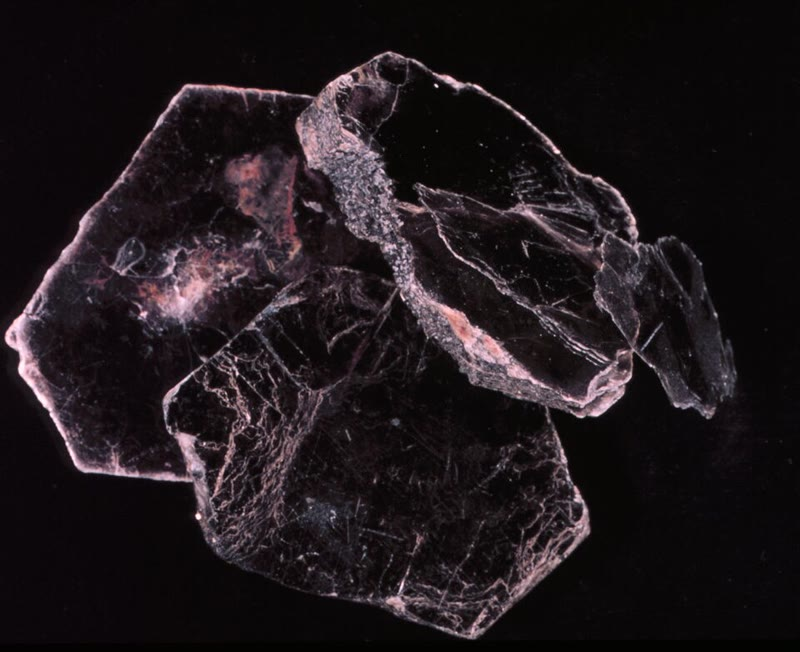
\includegraphics[height=2.75cm]{images/book2/g11-geodil-biotite.jpg}\hfill
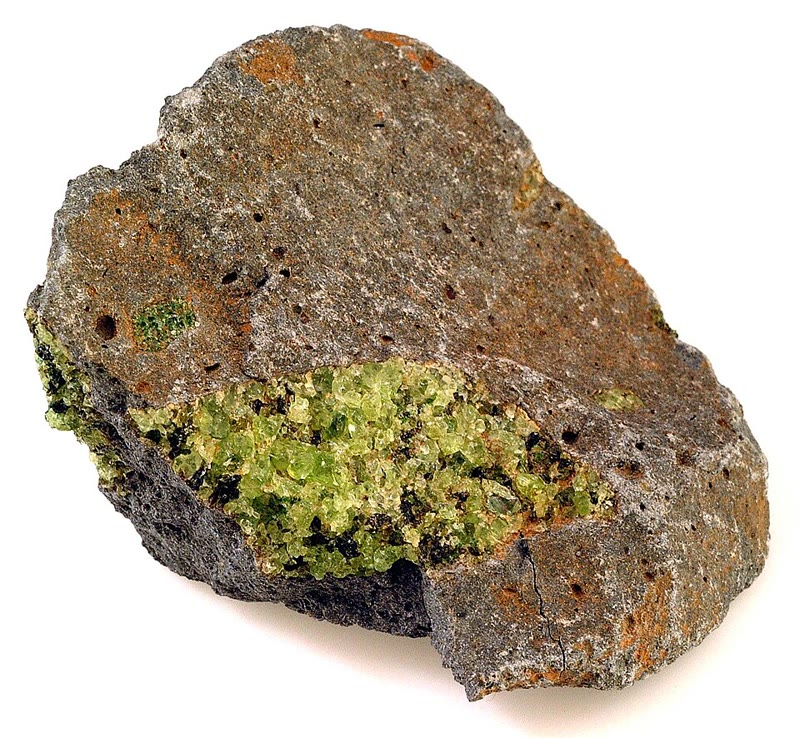
\includegraphics[height=2.75cm]{images/book2/g11-geodil-olivine.jpg}

{\small Four rock-forming minerals. From left to right: a quartz crystal,
a six-sided prism ending in points at both ends, about \qty{5}{cm} long; an
orthoclase feldspar, two crystals grown together, about \qty{7}{cm};
six-sided plates of biotite mica, about \qty{6}{cm}, which split into thin
sheets along their single \omterm{def:g11:minerals:cleavage}{cleavage}; green grains of olivine in a basalt.
Photographs Shannon Heinle, Darla Sondrol, Dexter Perkins and Nessa Eull,
Geology Digital Image Library (CC0).}
\end{omfigure}
% ledger: photo:g11-quartz, photo:g11-orthoclase, photo:g11-biotite, photo:g11-olivine

\section{Silicates}

\paragraph{Two elements make the crust.} The chemical composition of the
continental crust is known from the analyses of many rocks, reported as
percentages of oxides: about \qty{60.6}{\percent} \ce{SiO2},
\qty{15.9}{\percent} \ce{Al2O3}, and so on. From these, and from the masses of
the atoms, the mass of each element follows. Oxygen makes \qty{46}{\percent}
of the mass of the continental crust and silicon \qty{28}{\percent}: two
elements, about three quarters of the mass. With six metals --- aluminium,
iron, calcium, magnesium, sodium and potassium --- they make more than
\qty{99}{\percent} of it.
% ledger: rg14:crust, ciaaw:O, ciaaw:Si, ciaaw:Al, ciaaw:Fe, ciaaw:Ca, ciaaw:Mg, ciaaw:Na, ciaaw:K, ciaaw:Ti, ciaaw:Mn, ciaaw:P
% values (mineral_density.py): bulk_O 46.36, bulk_Si 28.30, O+Si 74.66, eight elements 99.43

\begin{omfigure}
\begin{tikzpicture}
\begin{axis}[omrecord, width=0.82\linewidth, height=5.6cm, ybar, bar width=14pt,
  ymin=0, ymax=55, xtick=data, enlarge x limits=0.06,
  xticklabels from table={figdata/out/grade-11-mineral_density-elements.dat}{symbol},
  ylabel={share of the mass (\unit{\percent})},
  nodes near coords, every node near coord/.append style={font=\scriptsize, /pgf/number format/.cd, fixed, precision=1},
  xmajorgrids=false]
% computed in figdata/grade-11/mineral_density.py; ledger: rg14:crust, ciaaw:*
\addplot[fill=omDef!55, draw=omDef] table[x expr=\coordindex, y=frac] {figdata/out/grade-11-mineral_density-elements.dat};
\end{axis}
\end{tikzpicture}

{\small The elements of the continental crust, as shares of its mass,
computed from its average composition in oxides (Rudnick and Gao, 2014).
Oxygen and silicon alone make about three quarters of the mass.}
\end{omfigure}

\paragraph{The silicon--oxygen tetrahedron.} A silicon atom is small, and
four oxygen atoms fit around it, at the corners of a tetrahedron, a pyramid
with four triangular faces. The group holds one silicon ion \ce{Si^4+} and
four oxygen ions \ce{O^2-}: it carries a charge of $4 - 4 \times 2 = -4$,
which other ions --- or other tetrahedra --- must balance.

\begin{definition}[Silicate; silicon--oxygen tetrahedron]\label{def:g11:minerals:silicate}
The \emph{silicon--oxygen tetrahedron}\index{silicon--oxygen tetrahedron} is
the group \ce{SiO4} formed by one silicon atom and the four oxygen atoms
around it, at the corners of a tetrahedron. A
\emph{silicate}\index{silicate} is a mineral built from silicon--oxygen
tetrahedra, alone or linked to one another by shared corners.
\end{definition}
% ledger: tulane:silicates

Tetrahedra link by sharing oxygens: the corner of one tetrahedron is the
corner of the next. How many corners each tetrahedron shares sets the
structure of the \omterm{def:g11:minerals:silicate}{silicate}, and its formula.
\begin{itemize}
  \item \emph{Isolated tetrahedra}, sharing no corner, held together by
        metal ions between them: olivine, \ce{(Mg,Fe)2SiO4}.
  \item \emph{Single chains}, each tetrahedron sharing two corners with its
        neighbours: the pyroxenes.
  \item \emph{Double chains}, two single chains joined side by side, the
        tetrahedra sharing two or three corners in turn: the amphiboles.
  \item \emph{Sheets}, each tetrahedron sharing three corners: the micas,
        and the \omterm{def:g10:soil-formation:clay}{clay minerals} of soils (\cref{ch:g10:soil-formation}).
  \item \emph{Frameworks}, each tetrahedron sharing all four corners, in all
        three directions of space: quartz, \ce{SiO2}, and --- with aluminium
        in place of some of the silicon --- the feldspars.
\end{itemize}
% ledger: tulane:silicates

\begin{omfigure}
\begin{tikzpicture}[font=\footnotesize]
  % coordinates generated once by a small script (scratch, not kept): kagome net of side 0.62 cm,
  % a regular tetrahedron in perspective, and a framework piece of five tetrahedra (painter's order)
  % (a) one SiO4 tetrahedron, drawn in perspective; the silicon (black) at its centre
  \fill[omDef!12] (2.300,2.979) -- (1.927,1.372) -- (1.221,0.629) -- (3.752,0.820) -- cycle;
  \draw[densely dashed, omDef!60, line width=0.6pt] (2.300,2.979) -- (1.927,1.372);
  \draw[omDef!70!black, line width=0.6pt] (2.300,2.979) -- (1.221,0.629);
  \draw[omDef!70!black, line width=0.6pt] (2.300,2.979) -- (3.752,0.820);
  \draw[densely dashed, omDef!60, line width=0.6pt] (1.927,1.372) -- (1.221,0.629);
  \draw[densely dashed, omDef!60, line width=0.6pt] (1.927,1.372) -- (3.752,0.820);
  \draw[omDef!70!black, line width=0.6pt] (1.221,0.629) -- (3.752,0.820);
  \draw[black!55, line width=0.4pt] (2.300,1.450) -- (2.300,2.979);
  \draw[black!55, line width=0.4pt] (2.300,1.450) -- (1.927,1.372);
  \draw[black!55, line width=0.4pt] (2.300,1.450) -- (1.221,0.629);
  \draw[black!55, line width=0.4pt] (2.300,1.450) -- (3.752,0.820);
  \fill[black] (2.300,1.450) circle (2.2pt);
  \filldraw[fill=omThm!35, draw=omThm!80!black, line width=0.4pt] (2.300,2.979) circle (4.2pt);
  \filldraw[fill=omThm!35, draw=omThm!80!black, line width=0.4pt] (1.927,1.372) circle (4.2pt);
  \filldraw[fill=omThm!35, draw=omThm!80!black, line width=0.4pt] (1.221,0.629) circle (4.2pt);
  \filldraw[fill=omThm!35, draw=omThm!80!black, line width=0.4pt] (3.752,0.820) circle (4.2pt);
  % coordinates for labels: Si 2.300,1.450; apex 2.300,2.979
  % (b) isolated tetrahedra (olivine)
  \filldraw[fill=omDef!22, draw=omDef!70!black, line width=0.5pt] (6.200,0.900) -- (6.820,0.900) -- (6.510,1.437) -- cycle;
  \fill[black] (6.510,1.079) circle (0.9pt);
  \filldraw[fill=omDef!22, draw=omDef!70!black, line width=0.5pt] (8.370,1.437) -- (8.990,1.437) -- (8.680,1.974) -- cycle;
  \fill[black] (8.680,1.616) circle (0.9pt);
  \filldraw[fill=omDef!22, draw=omDef!70!black, line width=0.5pt] (8.060,1.974) -- (7.750,2.511) -- (8.370,2.511) -- cycle;
  \fill[black] (8.060,2.332) circle (0.9pt);
  \filldraw[fill=omDef!22, draw=omDef!70!black, line width=0.5pt] (8.990,0.363) -- (9.610,0.363) -- (9.300,0.900) -- cycle;
  \fill[black] (9.300,0.542) circle (0.9pt);
  \filldraw[fill=omDef!22, draw=omDef!70!black, line width=0.5pt] (9.920,1.974) -- (9.610,2.511) -- (10.230,2.511) -- cycle;
  \fill[black] (9.920,2.332) circle (0.9pt);
  \filldraw[fill=omThm!35, draw=omThm!80!black, line width=0.4pt] (6.200,0.900) circle (1.9pt);
  \filldraw[fill=omThm!35, draw=omThm!80!black, line width=0.4pt] (6.510,1.437) circle (1.9pt);
  \filldraw[fill=omThm!35, draw=omThm!80!black, line width=0.4pt] (6.820,0.900) circle (1.9pt);
  \filldraw[fill=omThm!35, draw=omThm!80!black, line width=0.4pt] (7.750,2.511) circle (1.9pt);
  \filldraw[fill=omThm!35, draw=omThm!80!black, line width=0.4pt] (8.060,1.974) circle (1.9pt);
  \filldraw[fill=omThm!35, draw=omThm!80!black, line width=0.4pt] (8.370,2.511) circle (1.9pt);
  \filldraw[fill=omThm!35, draw=omThm!80!black, line width=0.4pt] (8.370,1.437) circle (1.9pt);
  \filldraw[fill=omThm!35, draw=omThm!80!black, line width=0.4pt] (8.680,1.974) circle (1.9pt);
  \filldraw[fill=omThm!35, draw=omThm!80!black, line width=0.4pt] (8.990,1.437) circle (1.9pt);
  \filldraw[fill=omThm!35, draw=omThm!80!black, line width=0.4pt] (9.610,2.511) circle (1.9pt);
  \filldraw[fill=omThm!35, draw=omThm!80!black, line width=0.4pt] (8.990,0.363) circle (1.9pt);
  \filldraw[fill=omThm!35, draw=omThm!80!black, line width=0.4pt] (9.300,0.900) circle (1.9pt);
  \filldraw[fill=omThm!35, draw=omThm!80!black, line width=0.4pt] (9.920,1.974) circle (1.9pt);
  \filldraw[fill=omThm!35, draw=omThm!80!black, line width=0.4pt] (10.230,2.511) circle (1.9pt);
  \filldraw[fill=omThm!35, draw=omThm!80!black, line width=0.4pt] (9.610,0.363) circle (1.9pt);
  % (c) single chain (pyroxenes)
  \filldraw[fill=omDef!22, draw=omDef!70!black, line width=0.5pt] (11.400,1.600) -- (12.020,1.600) -- (11.710,2.137) -- cycle;
  \fill[black] (11.710,1.779) circle (0.9pt);
  \filldraw[fill=omDef!22, draw=omDef!70!black, line width=0.5pt] (12.330,1.063) -- (12.020,1.600) -- (12.640,1.600) -- cycle;
  \fill[black] (12.330,1.421) circle (0.9pt);
  \filldraw[fill=omDef!22, draw=omDef!70!black, line width=0.5pt] (12.640,1.600) -- (13.260,1.600) -- (12.950,2.137) -- cycle;
  \fill[black] (12.950,1.779) circle (0.9pt);
  \filldraw[fill=omDef!22, draw=omDef!70!black, line width=0.5pt] (13.570,1.063) -- (13.260,1.600) -- (13.880,1.600) -- cycle;
  \fill[black] (13.570,1.421) circle (0.9pt);
  \filldraw[fill=omDef!22, draw=omDef!70!black, line width=0.5pt] (13.880,1.600) -- (14.500,1.600) -- (14.190,2.137) -- cycle;
  \fill[black] (14.190,1.779) circle (0.9pt);
  \filldraw[fill=omDef!22, draw=omDef!70!black, line width=0.5pt] (14.810,1.063) -- (14.500,1.600) -- (15.120,1.600) -- cycle;
  \fill[black] (14.810,1.421) circle (0.9pt);
  \filldraw[fill=omDef!22, draw=omDef!70!black, line width=0.5pt] (15.120,1.600) -- (15.740,1.600) -- (15.430,2.137) -- cycle;
  \fill[black] (15.430,1.779) circle (0.9pt);
  \filldraw[fill=omThm!35, draw=omThm!80!black, line width=0.4pt] (11.400,1.600) circle (1.9pt);
  \filldraw[fill=omThm!35, draw=omThm!80!black, line width=0.4pt] (11.710,2.137) circle (1.9pt);
  \filldraw[fill=omThm!35, draw=omThm!80!black, line width=0.4pt] (12.020,1.600) circle (1.9pt);
  \filldraw[fill=omThm!35, draw=omThm!80!black, line width=0.4pt] (12.330,1.063) circle (1.9pt);
  \filldraw[fill=omThm!35, draw=omThm!80!black, line width=0.4pt] (12.640,1.600) circle (1.9pt);
  \filldraw[fill=omThm!35, draw=omThm!80!black, line width=0.4pt] (12.950,2.137) circle (1.9pt);
  \filldraw[fill=omThm!35, draw=omThm!80!black, line width=0.4pt] (13.260,1.600) circle (1.9pt);
  \filldraw[fill=omThm!35, draw=omThm!80!black, line width=0.4pt] (13.570,1.063) circle (1.9pt);
  \filldraw[fill=omThm!35, draw=omThm!80!black, line width=0.4pt] (13.880,1.600) circle (1.9pt);
  \filldraw[fill=omThm!35, draw=omThm!80!black, line width=0.4pt] (14.190,2.137) circle (1.9pt);
  \filldraw[fill=omThm!35, draw=omThm!80!black, line width=0.4pt] (14.500,1.600) circle (1.9pt);
  \filldraw[fill=omThm!35, draw=omThm!80!black, line width=0.4pt] (14.810,1.063) circle (1.9pt);
  \filldraw[fill=omThm!35, draw=omThm!80!black, line width=0.4pt] (15.120,1.600) circle (1.9pt);
  \filldraw[fill=omThm!35, draw=omThm!80!black, line width=0.4pt] (15.430,2.137) circle (1.9pt);
  \filldraw[fill=omThm!35, draw=omThm!80!black, line width=0.4pt] (15.740,1.600) circle (1.9pt);
  % (d) double chain (amphiboles)
  \filldraw[fill=omDef!22, draw=omDef!70!black, line width=0.5pt] (0.600,-3.550) -- (1.220,-3.550) -- (0.910,-3.013) -- cycle;
  \fill[black] (0.910,-3.371) circle (0.9pt);
  \filldraw[fill=omDef!22, draw=omDef!70!black, line width=0.5pt] (1.530,-4.087) -- (1.220,-3.550) -- (1.840,-3.550) -- cycle;
  \fill[black] (1.530,-3.729) circle (0.9pt);
  \filldraw[fill=omDef!22, draw=omDef!70!black, line width=0.5pt] (1.840,-3.550) -- (2.460,-3.550) -- (2.150,-3.013) -- cycle;
  \fill[black] (2.150,-3.371) circle (0.9pt);
  \filldraw[fill=omDef!22, draw=omDef!70!black, line width=0.5pt] (2.770,-4.087) -- (2.460,-3.550) -- (3.080,-3.550) -- cycle;
  \fill[black] (2.770,-3.729) circle (0.9pt);
  \filldraw[fill=omDef!22, draw=omDef!70!black, line width=0.5pt] (3.080,-3.550) -- (3.700,-3.550) -- (3.390,-3.013) -- cycle;
  \fill[black] (3.390,-3.371) circle (0.9pt);
  \filldraw[fill=omDef!22, draw=omDef!70!black, line width=0.5pt] (4.010,-4.087) -- (3.700,-3.550) -- (4.320,-3.550) -- cycle;
  \fill[black] (4.010,-3.729) circle (0.9pt);
  \filldraw[fill=omDef!22, draw=omDef!70!black, line width=0.5pt] (4.320,-3.550) -- (4.940,-3.550) -- (4.630,-3.013) -- cycle;
  \fill[black] (4.630,-3.371) circle (0.9pt);
  \filldraw[fill=omDef!22, draw=omDef!70!black, line width=0.5pt] (0.910,-3.013) -- (0.600,-2.476) -- (1.220,-2.476) -- cycle;
  \fill[black] (0.910,-2.655) circle (0.9pt);
  \filldraw[fill=omDef!22, draw=omDef!70!black, line width=0.5pt] (1.220,-2.476) -- (1.840,-2.476) -- (1.530,-1.939) -- cycle;
  \fill[black] (1.530,-2.297) circle (0.9pt);
  \filldraw[fill=omDef!22, draw=omDef!70!black, line width=0.5pt] (2.150,-3.013) -- (1.840,-2.476) -- (2.460,-2.476) -- cycle;
  \fill[black] (2.150,-2.655) circle (0.9pt);
  \filldraw[fill=omDef!22, draw=omDef!70!black, line width=0.5pt] (2.460,-2.476) -- (3.080,-2.476) -- (2.770,-1.939) -- cycle;
  \fill[black] (2.770,-2.297) circle (0.9pt);
  \filldraw[fill=omDef!22, draw=omDef!70!black, line width=0.5pt] (3.390,-3.013) -- (3.080,-2.476) -- (3.700,-2.476) -- cycle;
  \fill[black] (3.390,-2.655) circle (0.9pt);
  \filldraw[fill=omDef!22, draw=omDef!70!black, line width=0.5pt] (3.700,-2.476) -- (4.320,-2.476) -- (4.010,-1.939) -- cycle;
  \fill[black] (4.010,-2.297) circle (0.9pt);
  \filldraw[fill=omDef!22, draw=omDef!70!black, line width=0.5pt] (4.630,-3.013) -- (4.320,-2.476) -- (4.940,-2.476) -- cycle;
  \fill[black] (4.630,-2.655) circle (0.9pt);
  \filldraw[fill=omThm!35, draw=omThm!80!black, line width=0.4pt] (0.600,-2.476) circle (1.9pt);
  \filldraw[fill=omThm!35, draw=omThm!80!black, line width=0.4pt] (0.600,-3.550) circle (1.9pt);
  \filldraw[fill=omThm!35, draw=omThm!80!black, line width=0.4pt] (0.910,-3.013) circle (1.9pt);
  \filldraw[fill=omThm!35, draw=omThm!80!black, line width=0.4pt] (1.220,-2.476) circle (1.9pt);
  \filldraw[fill=omThm!35, draw=omThm!80!black, line width=0.4pt] (1.530,-1.939) circle (1.9pt);
  \filldraw[fill=omThm!35, draw=omThm!80!black, line width=0.4pt] (1.220,-3.550) circle (1.9pt);
  \filldraw[fill=omThm!35, draw=omThm!80!black, line width=0.4pt] (1.840,-2.476) circle (1.9pt);
  \filldraw[fill=omThm!35, draw=omThm!80!black, line width=0.4pt] (1.530,-4.087) circle (1.9pt);
  \filldraw[fill=omThm!35, draw=omThm!80!black, line width=0.4pt] (1.840,-3.550) circle (1.9pt);
  \filldraw[fill=omThm!35, draw=omThm!80!black, line width=0.4pt] (2.150,-3.013) circle (1.9pt);
  \filldraw[fill=omThm!35, draw=omThm!80!black, line width=0.4pt] (2.460,-2.476) circle (1.9pt);
  \filldraw[fill=omThm!35, draw=omThm!80!black, line width=0.4pt] (2.770,-1.939) circle (1.9pt);
  \filldraw[fill=omThm!35, draw=omThm!80!black, line width=0.4pt] (2.460,-3.550) circle (1.9pt);
  \filldraw[fill=omThm!35, draw=omThm!80!black, line width=0.4pt] (3.080,-2.476) circle (1.9pt);
  \filldraw[fill=omThm!35, draw=omThm!80!black, line width=0.4pt] (2.770,-4.087) circle (1.9pt);
  \filldraw[fill=omThm!35, draw=omThm!80!black, line width=0.4pt] (3.080,-3.550) circle (1.9pt);
  \filldraw[fill=omThm!35, draw=omThm!80!black, line width=0.4pt] (3.390,-3.013) circle (1.9pt);
  \filldraw[fill=omThm!35, draw=omThm!80!black, line width=0.4pt] (3.700,-2.476) circle (1.9pt);
  \filldraw[fill=omThm!35, draw=omThm!80!black, line width=0.4pt] (4.010,-1.939) circle (1.9pt);
  \filldraw[fill=omThm!35, draw=omThm!80!black, line width=0.4pt] (3.700,-3.550) circle (1.9pt);
  \filldraw[fill=omThm!35, draw=omThm!80!black, line width=0.4pt] (4.320,-2.476) circle (1.9pt);
  \filldraw[fill=omThm!35, draw=omThm!80!black, line width=0.4pt] (4.010,-4.087) circle (1.9pt);
  \filldraw[fill=omThm!35, draw=omThm!80!black, line width=0.4pt] (4.320,-3.550) circle (1.9pt);
  \filldraw[fill=omThm!35, draw=omThm!80!black, line width=0.4pt] (4.630,-3.013) circle (1.9pt);
  \filldraw[fill=omThm!35, draw=omThm!80!black, line width=0.4pt] (4.940,-2.476) circle (1.9pt);
  \filldraw[fill=omThm!35, draw=omThm!80!black, line width=0.4pt] (4.940,-3.550) circle (1.9pt);
  % (e) sheet (micas)
  \filldraw[fill=omDef!22, draw=omDef!70!black, line width=0.5pt] (5.900,-4.100) -- (6.520,-4.100) -- (6.210,-3.563) -- cycle;
  \fill[black] (6.210,-3.921) circle (0.9pt);
  \filldraw[fill=omDef!22, draw=omDef!70!black, line width=0.5pt] (7.140,-4.100) -- (7.760,-4.100) -- (7.450,-3.563) -- cycle;
  \fill[black] (7.450,-3.921) circle (0.9pt);
  \filldraw[fill=omDef!22, draw=omDef!70!black, line width=0.5pt] (8.380,-4.100) -- (9.000,-4.100) -- (8.690,-3.563) -- cycle;
  \fill[black] (8.690,-3.921) circle (0.9pt);
  \filldraw[fill=omDef!22, draw=omDef!70!black, line width=0.5pt] (9.620,-4.100) -- (10.240,-4.100) -- (9.930,-3.563) -- cycle;
  \fill[black] (9.930,-3.921) circle (0.9pt);
  \filldraw[fill=omDef!22, draw=omDef!70!black, line width=0.5pt] (6.210,-3.563) -- (5.900,-3.026) -- (6.520,-3.026) -- cycle;
  \fill[black] (6.210,-3.205) circle (0.9pt);
  \filldraw[fill=omDef!22, draw=omDef!70!black, line width=0.5pt] (7.450,-3.563) -- (7.140,-3.026) -- (7.760,-3.026) -- cycle;
  \fill[black] (7.450,-3.205) circle (0.9pt);
  \filldraw[fill=omDef!22, draw=omDef!70!black, line width=0.5pt] (8.690,-3.563) -- (8.380,-3.026) -- (9.000,-3.026) -- cycle;
  \fill[black] (8.690,-3.205) circle (0.9pt);
  \filldraw[fill=omDef!22, draw=omDef!70!black, line width=0.5pt] (9.930,-3.563) -- (9.620,-3.026) -- (10.240,-3.026) -- cycle;
  \fill[black] (9.930,-3.205) circle (0.9pt);
  \filldraw[fill=omDef!22, draw=omDef!70!black, line width=0.5pt] (6.520,-3.026) -- (7.140,-3.026) -- (6.830,-2.489) -- cycle;
  \fill[black] (6.830,-2.847) circle (0.9pt);
  \filldraw[fill=omDef!22, draw=omDef!70!black, line width=0.5pt] (7.760,-3.026) -- (8.380,-3.026) -- (8.070,-2.489) -- cycle;
  \fill[black] (8.070,-2.847) circle (0.9pt);
  \filldraw[fill=omDef!22, draw=omDef!70!black, line width=0.5pt] (9.000,-3.026) -- (9.620,-3.026) -- (9.310,-2.489) -- cycle;
  \fill[black] (9.310,-2.847) circle (0.9pt);
  \filldraw[fill=omDef!22, draw=omDef!70!black, line width=0.5pt] (6.830,-2.489) -- (6.520,-1.952) -- (7.140,-1.952) -- cycle;
  \fill[black] (6.830,-2.131) circle (0.9pt);
  \filldraw[fill=omDef!22, draw=omDef!70!black, line width=0.5pt] (8.070,-2.489) -- (7.760,-1.952) -- (8.380,-1.952) -- cycle;
  \fill[black] (8.070,-2.131) circle (0.9pt);
  \filldraw[fill=omDef!22, draw=omDef!70!black, line width=0.5pt] (9.310,-2.489) -- (9.000,-1.952) -- (9.620,-1.952) -- cycle;
  \fill[black] (9.310,-2.131) circle (0.9pt);
  \filldraw[fill=omDef!22, draw=omDef!70!black, line width=0.5pt] (5.900,-1.952) -- (6.520,-1.952) -- (6.210,-1.415) -- cycle;
  \fill[black] (6.210,-1.773) circle (0.9pt);
  \filldraw[fill=omDef!22, draw=omDef!70!black, line width=0.5pt] (7.140,-1.952) -- (7.760,-1.952) -- (7.450,-1.415) -- cycle;
  \fill[black] (7.450,-1.773) circle (0.9pt);
  \filldraw[fill=omDef!22, draw=omDef!70!black, line width=0.5pt] (8.380,-1.952) -- (9.000,-1.952) -- (8.690,-1.415) -- cycle;
  \fill[black] (8.690,-1.773) circle (0.9pt);
  \filldraw[fill=omDef!22, draw=omDef!70!black, line width=0.5pt] (9.620,-1.952) -- (10.240,-1.952) -- (9.930,-1.415) -- cycle;
  \fill[black] (9.930,-1.773) circle (0.9pt);
  \filldraw[fill=omThm!35, draw=omThm!80!black, line width=0.4pt] (5.900,-1.952) circle (1.9pt);
  \filldraw[fill=omThm!35, draw=omThm!80!black, line width=0.4pt] (6.210,-1.415) circle (1.9pt);
  \filldraw[fill=omThm!35, draw=omThm!80!black, line width=0.4pt] (5.900,-3.026) circle (1.9pt);
  \filldraw[fill=omThm!35, draw=omThm!80!black, line width=0.4pt] (6.520,-1.952) circle (1.9pt);
  \filldraw[fill=omThm!35, draw=omThm!80!black, line width=0.4pt] (5.900,-4.100) circle (1.9pt);
  \filldraw[fill=omThm!35, draw=omThm!80!black, line width=0.4pt] (6.210,-3.563) circle (1.9pt);
  \filldraw[fill=omThm!35, draw=omThm!80!black, line width=0.4pt] (6.520,-3.026) circle (1.9pt);
  \filldraw[fill=omThm!35, draw=omThm!80!black, line width=0.4pt] (6.830,-2.489) circle (1.9pt);
  \filldraw[fill=omThm!35, draw=omThm!80!black, line width=0.4pt] (7.140,-1.952) circle (1.9pt);
  \filldraw[fill=omThm!35, draw=omThm!80!black, line width=0.4pt] (7.450,-1.415) circle (1.9pt);
  \filldraw[fill=omThm!35, draw=omThm!80!black, line width=0.4pt] (6.520,-4.100) circle (1.9pt);
  \filldraw[fill=omThm!35, draw=omThm!80!black, line width=0.4pt] (7.140,-3.026) circle (1.9pt);
  \filldraw[fill=omThm!35, draw=omThm!80!black, line width=0.4pt] (7.760,-1.952) circle (1.9pt);
  \filldraw[fill=omThm!35, draw=omThm!80!black, line width=0.4pt] (7.140,-4.100) circle (1.9pt);
  \filldraw[fill=omThm!35, draw=omThm!80!black, line width=0.4pt] (7.450,-3.563) circle (1.9pt);
  \filldraw[fill=omThm!35, draw=omThm!80!black, line width=0.4pt] (7.760,-3.026) circle (1.9pt);
  \filldraw[fill=omThm!35, draw=omThm!80!black, line width=0.4pt] (8.070,-2.489) circle (1.9pt);
  \filldraw[fill=omThm!35, draw=omThm!80!black, line width=0.4pt] (8.380,-1.952) circle (1.9pt);
  \filldraw[fill=omThm!35, draw=omThm!80!black, line width=0.4pt] (8.690,-1.415) circle (1.9pt);
  \filldraw[fill=omThm!35, draw=omThm!80!black, line width=0.4pt] (7.760,-4.100) circle (1.9pt);
  \filldraw[fill=omThm!35, draw=omThm!80!black, line width=0.4pt] (8.380,-3.026) circle (1.9pt);
  \filldraw[fill=omThm!35, draw=omThm!80!black, line width=0.4pt] (9.000,-1.952) circle (1.9pt);
  \filldraw[fill=omThm!35, draw=omThm!80!black, line width=0.4pt] (8.380,-4.100) circle (1.9pt);
  \filldraw[fill=omThm!35, draw=omThm!80!black, line width=0.4pt] (8.690,-3.563) circle (1.9pt);
  \filldraw[fill=omThm!35, draw=omThm!80!black, line width=0.4pt] (9.000,-3.026) circle (1.9pt);
  \filldraw[fill=omThm!35, draw=omThm!80!black, line width=0.4pt] (9.310,-2.489) circle (1.9pt);
  \filldraw[fill=omThm!35, draw=omThm!80!black, line width=0.4pt] (9.620,-1.952) circle (1.9pt);
  \filldraw[fill=omThm!35, draw=omThm!80!black, line width=0.4pt] (9.930,-1.415) circle (1.9pt);
  \filldraw[fill=omThm!35, draw=omThm!80!black, line width=0.4pt] (9.000,-4.100) circle (1.9pt);
  \filldraw[fill=omThm!35, draw=omThm!80!black, line width=0.4pt] (9.620,-3.026) circle (1.9pt);
  \filldraw[fill=omThm!35, draw=omThm!80!black, line width=0.4pt] (10.240,-1.952) circle (1.9pt);
  \filldraw[fill=omThm!35, draw=omThm!80!black, line width=0.4pt] (9.620,-4.100) circle (1.9pt);
  \filldraw[fill=omThm!35, draw=omThm!80!black, line width=0.4pt] (9.930,-3.563) circle (1.9pt);
  \filldraw[fill=omThm!35, draw=omThm!80!black, line width=0.4pt] (10.240,-3.026) circle (1.9pt);
  \filldraw[fill=omThm!35, draw=omThm!80!black, line width=0.4pt] (10.240,-4.100) circle (1.9pt);
  % (f) framework: a tetrahedron sharing all four corners
  \filldraw[fill=omThm!35, draw=omThm!80!black, line width=0.4pt] (12.990,-1.963) circle (2.1pt);
  \filldraw[fill=omThm!35, draw=omThm!80!black, line width=0.4pt] (12.896,-3.062) circle (2.1pt);
  \filldraw[fill=omDef!14, draw=omDef!70!black, line width=0.45pt, fill opacity=0.85] (12.896,-3.062) -- (12.990,-1.963) -- (12.299,-2.380) -- cycle;
  \filldraw[fill=omThm!35, draw=omThm!80!black, line width=0.4pt] (15.186,-2.119) circle (2.1pt);
  \filldraw[fill=omDef!14, draw=omDef!70!black, line width=0.45pt, fill opacity=0.85] (12.896,-3.062) -- (13.398,-2.458) -- (12.990,-1.963) -- cycle;
  \filldraw[fill=omThm!35, draw=omThm!80!black, line width=0.4pt] (15.092,-3.219) circle (2.1pt);
  \fill[black] (12.896,-2.466) circle (1.1pt);
  \filldraw[fill=omDef!34, draw=omDef!70!black, line width=0.45pt, fill opacity=0.85] (13.398,-2.458) -- (12.990,-1.963) -- (12.299,-2.380) -- cycle;
  \filldraw[fill=omDef!14, draw=omDef!70!black, line width=0.45pt, fill opacity=0.85] (15.092,-3.219) -- (15.186,-2.119) -- (14.496,-2.536) -- cycle;
  \filldraw[fill=omDef!25, draw=omDef!70!black, line width=0.45pt, fill opacity=0.85] (12.896,-3.062) -- (12.299,-2.380) -- (13.398,-2.458) -- cycle;
  \filldraw[fill=omDef!14, draw=omDef!70!black, line width=0.45pt, fill opacity=0.85] (15.092,-3.219) -- (15.595,-2.614) -- (15.186,-2.119) -- cycle;
  \fill[black] (15.092,-2.622) circle (1.1pt);
  \filldraw[fill=omThm!35, draw=omThm!80!black, line width=0.4pt] (12.299,-2.380) circle (2.1pt);
  \filldraw[fill=omDef!34, draw=omDef!70!black, line width=0.45pt, fill opacity=0.85] (15.595,-2.614) -- (15.186,-2.119) -- (14.496,-2.536) -- cycle;
  \filldraw[fill=omDef!25, draw=omDef!70!black, line width=0.45pt, fill opacity=0.85] (15.092,-3.219) -- (14.496,-2.536) -- (15.595,-2.614) -- cycle;
  \filldraw[fill=omThm!35, draw=omThm!80!black, line width=0.4pt] (13.398,-2.458) circle (2.1pt);
  \filldraw[fill=omThm!35, draw=omThm!80!black, line width=0.4pt] (14.496,-2.536) circle (2.1pt);
  \filldraw[fill=omDef!14, draw=omDef!70!black, line width=0.45pt, fill opacity=0.85] (13.900,-1.853) -- (14.496,-2.536) -- (13.398,-2.458) -- cycle;
  \filldraw[fill=omThm!35, draw=omThm!80!black, line width=0.4pt] (15.595,-2.614) circle (2.1pt);
  \filldraw[fill=omDef!14, draw=omDef!70!black, line width=0.45pt, fill opacity=0.85] (13.398,-2.458) -- (13.806,-2.953) -- (14.496,-2.536) -- cycle;
  \fill[black] (13.900,-2.450) circle (1.1pt);
  \filldraw[fill=omDef!22, draw=omDef!70!black, line width=0.45pt, fill opacity=0.85] (13.900,-1.853) -- (13.398,-2.458) -- (13.806,-2.953) -- cycle;
  \filldraw[fill=omDef!37, draw=omDef!70!black, line width=0.45pt, fill opacity=0.85] (13.900,-1.853) -- (13.806,-2.953) -- (14.496,-2.536) -- cycle;
  \filldraw[fill=omThm!35, draw=omThm!80!black, line width=0.4pt] (13.994,-0.754) circle (2.1pt);
  \filldraw[fill=omThm!35, draw=omThm!80!black, line width=0.4pt] (13.900,-1.853) circle (2.1pt);
  \filldraw[fill=omThm!35, draw=omThm!80!black, line width=0.4pt] (13.806,-2.953) circle (2.1pt);
  \filldraw[fill=omDef!14, draw=omDef!70!black, line width=0.45pt, fill opacity=0.85] (13.900,-1.853) -- (13.994,-0.754) -- (13.304,-1.171) -- cycle;
  \filldraw[fill=omDef!14, draw=omDef!70!black, line width=0.45pt, fill opacity=0.85] (13.900,-1.853) -- (14.402,-1.249) -- (13.994,-0.754) -- cycle;
  \filldraw[fill=omThm!35, draw=omThm!80!black, line width=0.4pt] (13.712,-4.053) circle (2.1pt);
  \fill[black] (13.900,-1.256) circle (1.1pt);
  \filldraw[fill=omDef!14, draw=omDef!70!black, line width=0.45pt, fill opacity=0.85] (13.712,-4.053) -- (13.806,-2.953) -- (13.116,-3.370) -- cycle;
  \filldraw[fill=omDef!34, draw=omDef!70!black, line width=0.45pt, fill opacity=0.85] (14.402,-1.249) -- (13.994,-0.754) -- (13.304,-1.171) -- cycle;
  \filldraw[fill=omDef!14, draw=omDef!70!black, line width=0.45pt, fill opacity=0.85] (13.712,-4.053) -- (14.214,-3.448) -- (13.806,-2.953) -- cycle;
  \filldraw[fill=omDef!25, draw=omDef!70!black, line width=0.45pt, fill opacity=0.85] (13.900,-1.853) -- (13.304,-1.171) -- (14.402,-1.249) -- cycle;
  \fill[black] (13.712,-3.456) circle (1.1pt);
  \filldraw[fill=omThm!35, draw=omThm!80!black, line width=0.4pt] (13.304,-1.171) circle (2.1pt);
  \filldraw[fill=omDef!34, draw=omDef!70!black, line width=0.45pt, fill opacity=0.85] (14.214,-3.448) -- (13.806,-2.953) -- (13.116,-3.370) -- cycle;
  \filldraw[fill=omDef!25, draw=omDef!70!black, line width=0.45pt, fill opacity=0.85] (13.712,-4.053) -- (13.116,-3.370) -- (14.214,-3.448) -- cycle;
  \filldraw[fill=omThm!35, draw=omThm!80!black, line width=0.4pt] (14.402,-1.249) circle (2.1pt);
  \filldraw[fill=omThm!35, draw=omThm!80!black, line width=0.4pt] (13.116,-3.370) circle (2.1pt);
  \filldraw[fill=omThm!35, draw=omThm!80!black, line width=0.4pt] (14.214,-3.448) circle (2.1pt);
  % labels
  \draw[black!60] (2.30,2.98) -- (3.35,3.25); \node[anchor=west] at (3.35,3.25) {oxygen};
  \draw[black!60] (2.30,1.45) -- (3.55,2.15); \node[anchor=west] at (3.55,2.15) {silicon};
  \node[align=center] at (2.3,-0.15) {(a) one tetrahedron, \ce{SiO4}};
  \node[align=center] at (8.2,-0.15) {(b) isolated tetrahedra:\\olivine};
  \node[align=center] at (13.5,-0.15) {(c) single chain:\\pyroxenes};
  \node[align=center] at (2.75,-4.85) {(d) double chain:\\amphiboles};
  \node[align=center] at (8.1,-4.85) {(e) sheet:\\micas};
  \node[align=center] at (13.9,-4.85) {(f) framework:\\quartz, feldspars};
\end{tikzpicture}

{\small (a) The \omterm{def:g11:minerals:silicate}{silicon--oxygen tetrahedron}: a silicon atom (black) and four
oxygen atoms (pink) at the corners of a tetrahedron. (b)--(e) Tetrahedra seen
from above, each as a triangle: the circles are the oxygens of its base, the
dot the silicon, beneath the fourth oxygen; two triangles meeting at a corner
share that oxygen. (f) In a framework every corner is shared, in three
dimensions: here one tetrahedron and its four neighbours. Drawings, not to
scale.}
\end{omfigure}
% ledger: tulane:silicates

\begin{proposition}[Counting the oxygens]\label{prop:g11:minerals:sharing}
In a \omterm{def:g11:minerals:silicate}{silicate} where each tetrahedron shares $n$ of its corners with other
tetrahedra, there are $4 - n/2$ oxygen atoms for each silicon atom. Isolated
tetrahedra give \ce{SiO4}, single chains \ce{SiO3}, sheets \ce{Si2O5} and
frameworks \ce{SiO2}.
\end{proposition}

\begin{proof}
Each tetrahedron has one silicon and four corners. A corner that is not
shared belongs to this tetrahedron alone and counts for one oxygen; a shared
corner belongs to two tetrahedra and counts for half an oxygen in each. With
$n$ shared corners, a tetrahedron owns $(4 - n) + n/2 = 4 - n/2$ oxygens.
For $n = 0$, $2$, $3$ and $4$ this gives $4$, $3$, $5/2$ and $2$ oxygens
per silicon: \ce{SiO4}, \ce{SiO3}, \ce{Si2O5} and \ce{SiO2}.
\end{proof}

The formulas of the minerals bear this out. The pyroxene augite contains
\ce{(Si,Al)2O6}, that is \ce{SiO3} twice, and the mica biotite \ce{AlSi3O10},
four tetrahedra for ten oxygens, \ce{Si2O5} twice; in a feldspar, four
tetrahedra hold eight oxygens, \ce{SiO2} four times, exactly as in quartz.
The charges, though, differ. Quartz is neutral: in a framework, each oxygen
is shared, and the charges of silicon and oxygen balance. In the other
structures the unshared oxygens carry spare negative charges, balanced by
metal ions --- magnesium and iron in olivine, potassium in orthoclase, where
one aluminium ion \ce{Al^3+} in place of a silicon ion \ce{Si^4+} leaves
one charge to be balanced.
% ledger: wm:densities (formulas)

\begin{definition}[Rock-forming silicates]\label{def:g11:minerals:rock-forming}
The \emph{rock-forming silicates}\index{rock-forming silicates} are the six
groups of \omterm{def:g11:minerals:silicate}{silicate} minerals that make up most common igneous and
metamorphic rocks: olivine, the pyroxenes, the amphiboles, the micas, the
feldspars and quartz. The feldspars are of two kinds: \emph{potassium
feldspar}, such as orthoclase, and \emph{plagioclase}, a series of
feldspars containing sodium and calcium.
\end{definition}
% ledger: tulane:silicates, wm:densities

\begin{center}
\small
\renewcommand{\arraystretch}{1.25}
\begin{tabular}{|l|l|l|c|}
\hline
\textbf{group (example)} & \textbf{structure} & \textbf{formula} & \textbf{density} \\
 & & & (\unit{g/cm^3}) \\
\hline
olivine & isolated tetrahedra & \ce{(Mg,Fe)2SiO4} & 3.32 \\
pyroxene (augite) & single chains & \ce{(Ca,Na)(Mg,Fe,Al,Ti)(Si,Al)2O6} & 3.4 \\
amphibole (hornblende) & double chains & \ce{Ca2[Mg4(Al,Fe)]Si7AlO22(OH)2} & 3.23 \\
mica (biotite) & sheets & \ce{K(Mg,Fe)3AlSi3O10(OH,F)2} & 3.09 \\
mica (muscovite) & sheets & \ce{KAl2(Si3Al)O10(OH,F)2} & 2.82 \\
potassium feldspar (orthoclase) & framework & \ce{KAlSi3O8} & 2.56 \\
plagioclase (oligoclase) & framework & \ce{(Na,Ca)(Si,Al)4O8} & 2.65 \\
quartz & framework & \ce{SiO2} & 2.62 \\
\hline
\end{tabular}

\smallskip
{\footnotesize The \omterm{def:g11:minerals:rock-forming}{rock-forming silicates}. Formulas and mean densities from
webmineral.com; a comma between two elements in brackets means that either
can take that place in the crystal.}
\end{center}
% ledger: wm:densities, tulane:silicates

The table holds a rule that runs through the rest of this book. The minerals
with isolated tetrahedra and chains, rich in iron and magnesium, are the
densest, above \qty{3.2}{g/cm^3}; the frameworks, made of silicon, aluminium,
sodium, potassium and calcium, are the lightest, about \qty{2.6}{g/cm^3}. The
micas lie between. Olivine and pyroxene make the \omterm{def:g11:ocean-ridges:peridotite}{peridotite} of the mantle;
feldspars and quartz, the granite of the continents: the light rock floats on
the dense one.
% ledger: wm:densities

\section{Minerals make rocks}

A rock is described first by its minerals and their proportions. Three rocks
met in earlier chapters show the range:
\begin{itemize}
  \item \emph{granite}: quartz, potassium feldspar and plagioclase, with a
        little biotite or muscovite --- the rock of the continents;
  \item \emph{basalt} and \emph{\omterm{def:g11:ocean-ridges:gabbro}{gabbro}}: plagioclase and pyroxene, often
        with olivine --- the rocks of the \omterm{def:g11:ocean-ridges:oceanic-lithosphere}{oceanic crust}, the first fine
        grained, the second coarse (\cref{ch:g11:igneous-rocks});
  \item \emph{\omterm{def:g11:ocean-ridges:peridotite}{peridotite}}: mostly olivine, with pyroxene --- the rock of the
        mantle.
\end{itemize}
% ledger: nps:granite-minerals, photo:g11-basalt-thin-section, photo:g11-olivine

\begin{omfigure}
\begin{tikzpicture}
\begin{axis}[omrecord, width=0.8\linewidth, height=6.4cm, xbar, bar width=8pt,
  xmin=2.4, xmax=3.5, ymin=-0.7, ymax=8.7, ytick={0,...,8},
  yticklabels={orthoclase, quartz, oligoclase, labradorite, muscovite, biotite, hornblende, olivine, augite},
  xlabel={density (\unit{g/cm^3})}, ymajorgrids=false, clip=false]
% computed in figdata/grade-11/mineral_density.py (density_order); ledger: wm:densities
\addplot[fill=omDef!45, draw=omDef] table[x=rho, y=idx] {figdata/out/grade-11-mineral_density-densities.dat};
\draw[omProp, line width=1pt, dashed] (axis cs:2.6427,-0.7) -- (axis cs:2.6427,8.7) node[above, text height=1.6ex, text depth=0.3ex, font=\scriptsize, text=omProp!80!black] {granite};
\draw[omThm, line width=1pt, dashed] (axis cs:3.0015,-0.7) -- (axis cs:3.0015,8.7) node[above, text height=1.6ex, text depth=0.3ex, font=\scriptsize, text=omThm] {basalt};
\draw[black!70, line width=1pt, dashed] (axis cs:3.34,-0.7) -- (axis cs:3.34,8.7) node[above, font=\scriptsize] {peridotite};
\end{axis}
\end{tikzpicture}

{\small The mean densities of nine rock-forming minerals (webmineral.com),
and the densities of the three example rocks of this section computed with
the proposition below (dashed lines): a granite of quartz, feldspars and
micas, a basalt of plagioclase, pyroxene and some olivine, a \omterm{def:g11:ocean-ridges:peridotite}{peridotite} of
olivine and pyroxene.}
\end{omfigure}
% values (mineral_density.py): rho_granite 2.6427, rho_basalt 3.0015, rho_peridotite 3.34

The density of a rock follows from its minerals. Imagine a block of rock of
volume $V$, a fraction $\phi_1$ of it made of a first mineral, $\phi_2$ of a
second, and so on.

\begin{proposition}[The density of a rock from its minerals]\label{prop:g11:minerals:density}
A rock without pores, made of minerals of densities $\rho_1, \rho_2, \dots,
\rho_k$ occupying fractions $\phi_1, \phi_2, \dots, \phi_k$ of its volume
($\phi_1 + \dots + \phi_k = 1$), has the density
\[
  \rho = \phi_1 \rho_1 + \phi_2 \rho_2 + \dots + \phi_k \rho_k ,
\]
the mean of the densities of its minerals, weighted by their volume
fractions.
\end{proposition}

\begin{proof}
In a volume $V$ of rock, mineral $i$ occupies the volume $\phi_i V$ and has
the mass $\rho_i \phi_i V$. With no pores, the mass of the rock is the sum of
these masses, $m = (\phi_1 \rho_1 + \dots + \phi_k \rho_k)\,V$, and its
density is $m/V$.
\end{proof}

How are the volume fractions measured? On a flat cut face of the rock, or on
a \omterm{def:g11:minerals:thin-section}{thin section} (next section), a regular grid of points is laid out, and at
each point the mineral beneath is noted. When the grains are scattered
without order, the fraction of the points that fall on a mineral estimates
the fraction of the area it covers, and that is also the fraction of the
volume it fills: a thin slice is a fair sample of the whole block. This is a
\emph{point count}.

\begin{example}[A granite light in quartz and potassium feldspar]
A point count gives \qty{35}{\percent} quartz (\qty{2.62}{g/cm^3}),
\qty{50}{\percent} orthoclase (\qty{2.56}{g/cm^3}) and \qty{15}{\percent}
oligoclase (\qty{2.65}{g/cm^3}). The density of the rock is
\[
  \rho = 0.35 \times 2.62 + 0.50 \times 2.56 + 0.15 \times 2.65
       = 0.917 + 1.280 + 0.398 \approx \qty{2.59}{g/cm^3}.
\]
Measurements bear out this order of magnitude: of \num{6454} rock samples
weighed from about two hundred bodies of granitic rock in the Sierra Nevada of
California, the average is \qty{2.69}{g/cm^3}, and the granites richest in
silica and potassium, like this one, are below \qty{2.6}{g/cm^3}.
\end{example}
% ledger: wm:densities, usgs91:sierra

\section{Thin sections}

A hand lens shows grains a millimetre across. To see finer grains, and to
identify them with certainty, geologists look at rocks through a microscope
--- not at their surface, but through them.

\begin{definition}[Thin section; polarising microscope]\label{def:g11:minerals:thin-section}
A \emph{thin section}\index{thin section} is a slice of rock ground down to
a thickness of \qty{0.03}{mm} and mounted on a glass slide: at this thickness
light passes through most minerals. A \emph{polarising
microscope}\index{polarising microscope} is a microscope fitted with two
polarising filters, one below the slide and one above it. The section is
seen in \emph{plane-polarised light} with the lower filter only, and between
\emph{crossed polars} when the upper filter is added with its direction
perpendicular to that of the lower one.
\end{definition}
% ledger: tulane:thin-section

\begin{omfigure}
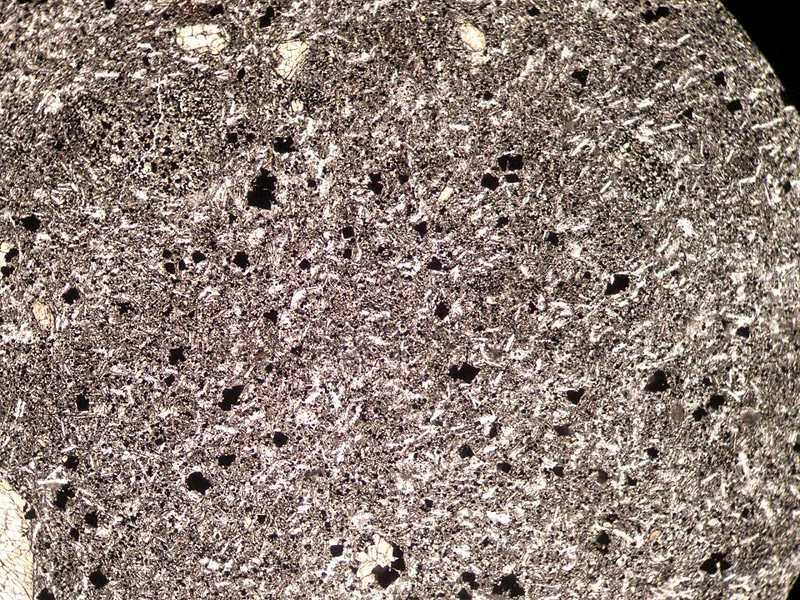
\includegraphics[height=3.6cm]{images/book2/g11-chmee2-basalt-ppl.jpg}\hfill
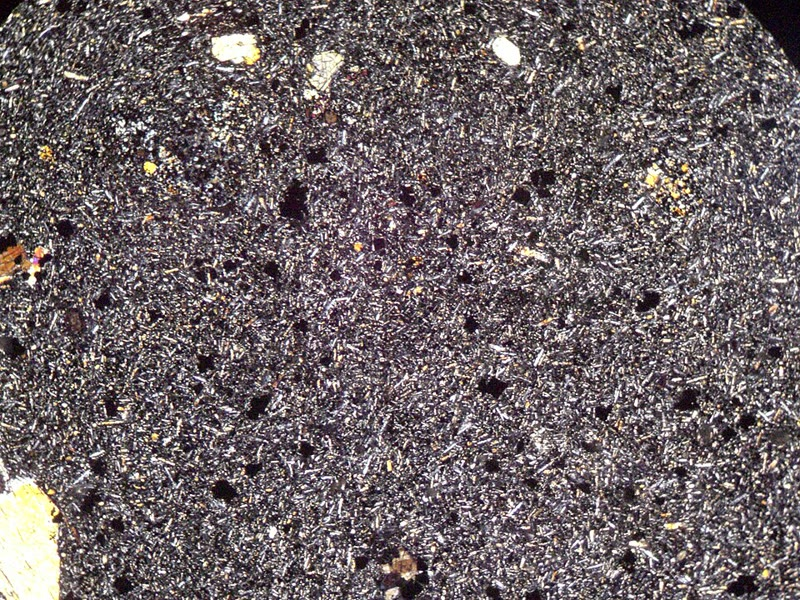
\includegraphics[height=3.6cm]{images/book2/g11-chmee2-basalt-xpl.jpg}\hfill
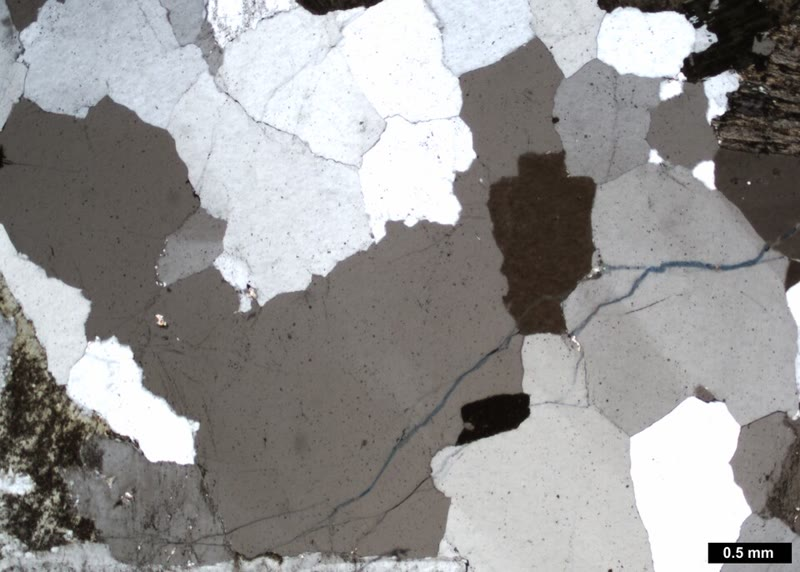
\includegraphics[height=3.6cm]{images/book2/g11-rygel-granite-xpl.jpg}

{\small Left and centre: the same basalt in \omterm{def:g11:minerals:thin-section}{thin section}, in plane-polarised
light and between crossed polars. The rock is fine grained: small elongated
crystals, mostly plagioclase, and black specks that let no light through in
either view; between crossed polars the crystals light up in greys and
colours. Photographs
Chmee2 (CC~BY-SA~3.0). Right: crystals of quartz in a granite, between
crossed polars, each in its own shade of grey (the scale bar is
\qty{0.5}{mm}). Photograph Michael C.~Rygel (CC~BY-SA~3.0).}
\end{omfigure}
% ledger: photo:g11-basalt-thin-section, photo:g11-granite-thin-section

In plane-polarised light a \omterm{def:g11:minerals:thin-section}{thin section} looks like a stained-glass window:
most minerals are nearly colourless, some tinted, and the outlines of the
grains, their \omterm{def:g11:minerals:cleavage}{cleavages} and their \omterm{def:g11:minerals:habit}{habits} show sharply. Between crossed
polars the filters, set across each other, would let no light through
on their own; most minerals alter the light that crosses them, and appear
in shades of grey or in bright colours, which change as the slide is turned.
Two grains of the same mineral can look different, because each is cut in
its own direction: the quartz grains of the granite above are all quartz,
in different shades. The colours, how they change, and what they reveal
about each mineral are the subject of the first university year; here, the
\omterm{def:g11:minerals:thin-section}{thin section} is a picture of the rock, in which every grain can be seen,
named and counted.

\section{Exercises}

\begin{exercise}[$\star$]\label{exo:g11:minerals:1}
Define \omterm{def:g11:minerals:cleavage}{cleavage} and fracture. Which one does quartz show, and what do its
broken surfaces look like? How many \omterm{def:g11:minerals:cleavage}{cleavages} does a mica have?
\end{exercise}

\begin{exercise}[$\star$]\label{exo:g11:minerals:2}
Why is colour a poor guide to identifying quartz, but a fairly good one for
olivine? Give two properties more reliable than colour.
\end{exercise}

\begin{exercise}[$\star$]\label{exo:g11:minerals:3}
Match each description to a mineral among quartz, orthoclase, biotite and
olivine: (1) green grains in a basalt; (2) black flakes that peel into thin
sheets; (3) pink blocky grains with two flat breakage planes, scratched by a
steel nail; (4) glassy grey grains with curved breaks, not scratched by the
nail.
\end{exercise}

\begin{exercise}[$\star$]\label{exo:g11:minerals:4}
(1) How many atoms does a \omterm{def:g11:minerals:silicate}{silicon--oxygen tetrahedron} contain, and where are
they? (2) Using the charges of the ions \ce{Si^4+} and \ce{O^2-}, find the
charge of the group \ce{SiO4}.
\end{exercise}

\begin{exercise}[$\star$]\label{exo:g11:minerals:5}
Name the six groups of \omterm{def:g11:minerals:rock-forming}{rock-forming silicates} and give, for each, the way
its tetrahedra are linked.
\end{exercise}

\begin{exercise}[$\star\star$]\label{exo:g11:minerals:6}
The atomic masses of silicon and oxygen are \qty{28.085}{g/mol} and
\qty{15.999}{g/mol}. (1) Compute the share of oxygen in the mass of quartz,
\ce{SiO2}. (2) Do the same for forsterite, the magnesium olivine
\ce{Mg2SiO4} (magnesium: \qty{24.305}{g/mol}). (3) Compare with the share of
oxygen in the continental crust, about \qty{46}{\percent}.
\end{exercise}

\begin{exercise}[$\star\star$]\label{exo:g11:minerals:7}
A white grain in a granite scratches a glass plate (about 5.5) but is
scratched by a steel nail (about 6.5); it breaks along flat planes in two
directions. A second, grey grain is not scratched by the nail and breaks
along curved surfaces. Identify both, giving the reasons.
\end{exercise}

\begin{exercise}[$\star\star$]\label{exo:g11:minerals:8}
In the pyroxene augite, each tetrahedron shares two corners. (1) Using the
proposition on counting the oxygens, how many oxygens are there for each
silicon? (2) Check that the part \ce{(Si,Al)2O6} of the formula of augite
agrees.
\end{exercise}

\begin{exercise}[$\star\star$]\label{exo:g11:minerals:9}
A basalt is made of \qty{55}{\percent} labradorite (\qty{2.69}{g/cm^3}),
\qty{35}{\percent} augite (\qty{3.4}{g/cm^3}) and \qty{10}{\percent} olivine
(\qty{3.32}{g/cm^3}), by volume. Compute its density, then the mass of a
cube of this basalt \qty{10}{cm} on a side.
\end{exercise}

\begin{exercise}[$\star\star$]\label{exo:g11:minerals:10}
A \omterm{def:g11:ocean-ridges:peridotite}{peridotite} of the mantle is made of \qty{75}{\percent} olivine
(\qty{3.32}{g/cm^3}) and \qty{25}{\percent} augite (\qty{3.4}{g/cm^3}).
(1) Compute its density. (2) By what percentage is it denser than the
basalt of the previous exercise, at about \qty{3.00}{g/cm^3}? (3) Why does
the \omterm{def:g11:ocean-ridges:oceanic-lithosphere}{oceanic crust} stay on top of the mantle?
\end{exercise}

\begin{exercise}[$\star\star$]\label{exo:g11:minerals:11}
On a \omterm{def:g11:minerals:thin-section}{thin section} of a rock, a grid of 400 points falls 168 times on
plagioclase, 132 times on pyroxene, 60 times on olivine and 40 times on
holes left by gas bubbles. (1) Compute the fraction of each. (2) Why can the
proposition on the density of a rock not be applied directly to the whole
section? (3) Compute the density of the solid part, with \qty{2.69}{},
\qty{3.4}{} and \qty{3.32}{g/cm^3}, then that of the rock with its holes.
\end{exercise}

\begin{exercise}[$\star\star\star$]\label{exo:g11:minerals:12}
In \qty{1}{kg} of continental crust there are about \qty{464}{g} of oxygen,
\qty{283}{g} of silicon, \qty{84}{g} of aluminium, \qty{52}{g} of iron,
\qty{46}{g} of calcium, \qty{28}{g} of magnesium, \qty{23}{g} of sodium and
\qty{15}{g} of potassium. The atomic masses are \qty{16.0}{}, \qty{28.1}{},
\qty{27.0}{}, \qty{55.8}{}, \qty{40.1}{}, \qty{24.3}{}, \qty{23.0}{} and
\qty{39.1}{g/mol}. (1) Compute the number of moles of each element. (2) What
fraction of the atoms of the crust are oxygen atoms? (3) Why is the crust
sometimes described as a packing of oxygen ions, with the other elements in
the spaces between them?
\end{exercise}

\begin{exercise}[$\star\star\star$]\label{exo:g11:minerals:13}
In an amphibole double chain, half of the tetrahedra share two corners and
half share three. (1) How many oxygens are there for each silicon? (2) Write
the result for four silicons. (3) In the formula of hornblende,
\ce{Ca2[Mg4(Al,Fe)]Si7AlO22(OH)2}, aluminium takes the place of silicon in
one tetrahedron out of eight. Check that the formula agrees.
\end{exercise}

\begin{exercise}[$\star\star\star$]\label{exo:g11:minerals:14}
Over the Sierra Nevada of California, \num{6454} granitic rock samples have
an average density of \qty{2.69}{g/cm^3}; it is above \qty{2.7}{g/cm^3} in
the west, and below \qty{2.6}{g/cm^3} where the granite is richest in silica
and potassium. Compute the density of a rock of \qty{20}{\percent} quartz
(\qty{2.62}{g/cm^3}), \qty{10}{\percent} orthoclase (\qty{2.56}{}),
\qty{50}{\percent} oligoclase (\qty{2.65}{}), \qty{10}{\percent} biotite
(\qty{3.09}{}) and \qty{10}{\percent} hornblende (\qty{3.23}{}). Compare
with the granite of the example of this chapter, and explain the contrast
between the two parts of the Sierra Nevada.
\end{exercise}

\begin{exercise}[$\star\star\star$]\label{exo:g11:minerals:15}
The upper continental crust contains about \qty{66.6}{\percent} \ce{SiO2}
by mass, the continental crust as a whole \qty{60.6}{\percent}. (1) Using
the share of silicon in \ce{SiO2} (\qty{46.7}{\percent}), compute the share
of silicon held in \ce{SiO2} in each. (2) Which minerals would you expect to
be more common in the upper crust than lower down? (3) What does this imply
for the density of the upper crust compared with the deeper crust?
\end{exercise}

\section{Problem: The Density of a Granite}

\begin{problem}[{Weekend problem --- from a point count to a density}]
\label{pb:g11:minerals:1}
% values (mineral_density.py): GRANITE_COUNT 150/175/125/30/20; rho_granite 2.6427;
% granite_air_g 264.27, granite_water_g 164.27; densities wm:densities; usgs91:sierra
A block of pink granite is cut and polished. Its minerals are identified,
counted on a grid, and the density of the rock is computed, then checked by
weighing.

\medskip
\noindent\textbf{Part I --- Identifying the minerals.}
\begin{enumerate}
  \item Grains A are grey and glassy, show no flat breakage surface, only
        curved ones, and are not scratched by a steel nail. Which mineral
        are they?
  \item Grains B are pink and blocky, break along flat shining planes in
        two directions, scratch glass but are scratched by the nail. Which
        mineral are they, and what is their hardness on the Mohs scale?
  \item Grains C have the same hardness and \omterm{def:g11:minerals:cleavage}{cleavages} as grains B but are
        white; an analysis finds sodium and calcium in them, and no
        potassium. Which kind of feldspar are they?
  \item Grains D are black flakes, grains E silvery flakes; both peel into
        thin sheets. Which minerals are they, and which feature of their
        structure explains the sheets?
  \item Which of the minerals A to E are framework \omterm{def:g11:minerals:silicate}{silicates}? Which contain
        iron and magnesium?
\end{enumerate}

\medskip
\noindent\textbf{Part II --- The point count.}
\begin{enumerate}[resume]
  \item A grid of 500 points falls 150 times on quartz, 175 times on
        orthoclase, 125 times on oligoclase, 30 times on biotite and 20 times
        on muscovite. Compute the fraction of each mineral.
  \item Why does the fraction of points estimate the fraction of the volume
        of the rock?
  \item What percentage of the rock is feldspar?
  \item If one point is wrongly counted, by how much does a fraction change?
  \item Is this rock a granite in the sense of Book 1?
\end{enumerate}

\medskip
\noindent\textbf{Part III --- The density.}
\begin{enumerate}[resume]
  \item State the formula giving the density of a rock without pores from
        its minerals.
  \item With the densities quartz \qty{2.62}{}, orthoclase \qty{2.56}{},
        oligoclase \qty{2.65}{}, biotite \qty{3.09}{} and muscovite
        \qty{2.82}{g/cm^3}, compute the contribution $\phi_i \rho_i$ of
        each mineral.
  \item Add them up: what is the density of the granite?
  \item Which mineral contributes most to the sum? Which two minerals,
        though they make only a tenth of the rock, raise its density?
  \item Convert the density to \unit{kg/m^3}, and give the mass of
        \qty{1}{m^3} of this granite.
\end{enumerate}

\medskip
\noindent\textbf{Part IV --- Checking by weighing.}
\begin{enumerate}[resume]
  \item A block of \qty{100}{cm^3} is cut from the granite. What mass do you
        expect it to have?
  \item Hung in water, a body is pushed up by the weight of the water it
        displaces (physics). What mass does the balance read when the block
        hangs fully immersed in water, of density \qty{1.00}{g/cm^3}?
  \item Laboratories compute the density of a rock sample as
        $m_{\text{air}}/(m_{\text{air}} - m_{\text{water}})$. Check that
        your two masses give back the density of question~13.
  \item Granitic rocks of the Sierra Nevada average \qty{2.69}{g/cm^3}, and
        those richest in silica and potassium lie below \qty{2.6}{g/cm^3}.
        Where does this granite lie, and which minerals would make a
        granite denser?
  \item Conclude: what is the density of the granite?
\end{enumerate}
\end{problem}
